This section has the important role of listing methods for High-Speed ADC evaluation and sub-ADC evaluation. For an ADC, both static and dynamic performances shall be known for practical use case. In our case, we limit the scope of metric to those listed in the Table~\ref{tbl:adc-metric-subset}.

Classical methods are now mainstream in the industry and can be found in application notes of some manufacturer~\cite{AD-AN835,TI-SBAA002A,AD-DCH2005}. Several methodologies existing, they are gathered on the criterion of whether they are for static metrics or dynamic ones. For each, the mean to extract the metric listed in the Table~\ref{tbl:adc-metric-subset} is discussed.

Since the ADC IP bloc is differential others metrics are of interest such as:
\begin{itemize}
    \item Common mode and differential input impedance1
    \item maximum common-mode signal
    \item maximum operating common-mode signal
    \item common-mode rejection ratio
    \item common-mode out-of-range
\end{itemize}
These are not discussed in this section.

\begin{table}[htp]
    \centering
    \caption{Metric of interest for the ADC tests}
    \label{tbl:adc-metric-subset}
    \begin{tabular}{l|l}
        \toprule
        \textbf{Static Metric} & \textbf{Dynamic Metric} \\ \midrule
        -- Gain Error & -- Single-Tone Signal to Noise Ratio (SNR)\\
        -- Offset Error & -- Signal to Noise and Distortion (SINAD)\\
        -- Temperature Drift of Gain and Offset Error & -- Effective Number of Bits (ENOB)\\
        -- Differential Non Linearity (DNL) & -- Total Harmonic Distortion (THD) \\
        -- Integral Non Linearity (INL) & \\ \bottomrule
    \end{tabular}
\end{table}

\subsection{IEEE recommendations}
    \subsubsection{Static Metric}
Among static metrics extraction methods, the histogram based is widely adapted. An histogram is collected by driving the analogue inputs of the ADC with a known signal. Each bin value of the histogram corresponds to how many times the associated code of this bin is counted. The offset of the ADC can be estimated as the average code of all if the input signals applied have a zero mean. The offset error is thus, the difference between the average output code and the ideal output code. The gain error defined as the ratio of the actual transfer function slope over the ideal one can be seen on the histogram as a discrepancy between the first and the last bins weight and their ideal weight. For instance, a slope coefficient lower than the ideal one (negative gain error) will display an histogram close to the ideal one shrink into fewer bins and extreme bins values higher than expected as depicted by the \figurename~\ref{fig:gain-error-hist}.

\begin{figure}[htp]
    \centering
    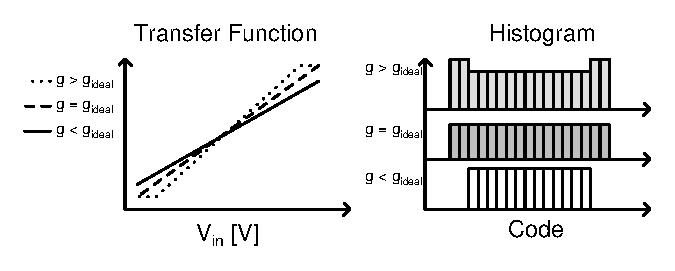
\includegraphics[width=0.8\textwidth]{Chapter5/Figs/sar_test/histogram_gain_error.ps}
    \caption{Gain error detection in an histogram based analysis}
    \label{fig:gain-error-hist}
\end{figure}

The input signal can be a ramp, a sine wave, or small signal variation around an even increasing offset, the DNL and INL can be extracted by subtracting the actual ADC histogram to the ideal ADC histogram. In a practical implementation, the input stimulus might not be perfectly linear and might degrade the DNL estimation. As a common practice, the stimulus linearity is 2 to 3 bits higher than the ADC under test. The INL is usually defined as the cumulative sum of the DNL\@. To limit the number of record a ramp is usually preferred. A sine wave can be applied to reduce the test time but the number of records should be selected as described at the page 41 of~\cite{IEEESTD1241-2010}.

A major flaw of this testing method concerns potential missing codes. Since the histogram is a counter of code occurrence, the occurrence of a missing code is attributed to the closest adjacent code. So an incorrect amount of occurrences is detectable but this implies that we are not able to detect a missing code. To avoid these issues, the ADC should also be tested for SINAD performance to confirm that non-monotonic behaviour is not significant.

By applying a signal on the ADC inputs, the output codes should ideally represents the input signal applied. Therefore, a fitting of output codes with the ideally expected results is sufficient to extract the gain and the offset of the ADC under test. The input signal can be either a ramp or a sine wave, and a least mean square algorithm is able to extract errors on the gain and the offset.
Unfortunately, this method is input dependant, and does not extract other metrics. A classical post-processing of output codes is necessary to extract dynamic characteristic and non-linearity (histogram, FFT). Its advantage over the method in the previous clause is that it is less sensitive to noise and more thoroughly eliminates spectral leakage.

However, the transfer function of an ADC can also be estimated by knowing at which input voltages occurs a transition. The servo-loop method is a closed loop approached consisting in finding the code transition level of a given reference code. This method is well suited to find transition in the transfer function.
An ADC output code different from the one selected will adjust the ADC input voltage until the reference code is met. Once the code transition level has been reached, the input signal is forced to oscillate across this transition.
This time the input voltage should be measured with an extra difficulty coming from the final oscillations. Either filtering or averaging is necessary with a bias correction to determine the ideal voltage value. Repeating this process for each code of the ADC, the INL can be estimated from all the ideal voltage value.
The input stimulus can be generated by either a DAC at the input. In which all the estimation is digital. Or the input voltage is done by an analogue integrator. This method is limited by the confidence in the linearity and the performances of the DAC used.

    \subsubsection{Dynamic Metric}
The dynamic metrics are usually extracted from the FFT of the sine wave reconstructed~\cite{IEEESTD1241-2010}. Nevertheless, some precautions on the signal have to be respected: the number of records and the frequency of the single-tone sine wave are only two among many.
For high speed ADC, the IEEE standard 1241-2010 recommends the use of a memory buffer to acquire data at the ADC sample rate. While the coherent sampling is reached when there is an integer number of waveform cycles in the data record. The following relationship describes it:
    \begin{equation}
        M F_i = J F_s
    \end{equation}
Where Fs is the sampling frequency, J is the integer number of cycles of the waveform in the data record, Fi is the frequency of the input waveform, and M is the number of samples in the data record. The recommendation is to set J to be at least 5 and to be co-prime with M. ($J = 5$, $M = 7\times2^{12}$ are co-prime)

Concerning the distortion of the input sine wave, the THD should be far less than the one of the expected ADC\@. Otherwise, this non-linearity will be found as well in the INL plot as in the dynamic parameters. The purity of the sine wave should be ensured and readily tested with a spectrum analyser.
The clear advantage of the sine wave stimulus is the relax constraint on the signal and clock synchronicity. The trigger of conversion does not have to be synchronized.
Finally, a great care is considered about the input signal overdrive which should at least be 3 times the rms value of the random noise at the input. If noise is present, it will modify the probabilities of samples falling in various code bins, and the effect will be largest near the peaks where the curvature of the probability density is greatest.
Once the setup configured, the metrics are extracted from the FFT of the reconstructed signal. To prevent spectral leakage, a rectangular window is sufficient if the coherent sampling criterion is respected (a single ray at the input frequency shall be present in the spectrum). Otherwise, whatsoever the window is applied the record length should large enough to reduce the spectral leakage.

% \subsection{Application to the ADC}
% As recommended by the IEEE standard 1241-2010~\cite{IEEESTD1241-2010}, and by comparison of existing technique presented earlier, in both the static and dynamic testing, the input stimulus will be a sinusoid. This demonstrates a clear advantage on the testing time by performing a single test and being able to characterize both the static and the dynamic of the ADC\@.
% There must be an exact integer number of cycles in a record, and the number of cycles in a record must be relatively prime to the number of samples in the record. This guarantees that the samples in each record are uniformly distributed in phase from 0 to 2$\pi$. Assuming the noise power of the signal generator to be, the sine wave excursion should be  where  is the differential input voltage range of the stage under test.
% The sine wave is selected for its ease of realization with respect to the linearity required to be about 16 bits. In this regards, the coherent sampling parameters for an accurate DNL/INL estimation to 0.1 LSB, should be tuned as follows:
% \begin{itemize}
%     \item number of cycle in a unit record: J should be any odd number below M/2
%     \item number of data in a unit record: M = 32
%     \item sampling frequency: fs = 20 MHz
%     \item input signal frequency: f = fs J/M
%     \item $\frac{F_s}{F} d\left(\frac{F}{F_s}\right) \leq \frac{1}{4M(J-1)}$ (the chosen M allows for an error of 5.4 kHz on the input signal frequency
%     \item total number of record for 0.01 LSB accuracy of 14 bits ADC INL/DNL\@: > 772 078 (closest integer multiple of M is 772 096 for 24128 unit record).
% \end{itemize}

% The tests should be done from -40\(\degree\)C to +175\(\degree\)C at least at the following 10 temperatures:
% \begin{multicols}{2}
%     \begin{itemize}
%         \item -40\(\degree\)C
%         \item -25\(\degree\)C
%         \item 0\(\degree\)C
%         \item 27\(\degree\)C
%         \item 62\(\degree\)C
%         \item 85\(\degree\)C
%         \item 100\(\degree\)C
%         \item 125\(\degree\)C
%         \item 150\(\degree\)C
%         \item 175\(\degree\)C
%     \end{itemize}
% \end{multicols}

% The accuracy of analogue voltage, at the exception of power supplies, should be of 400 $\mu$V. For the power supply, the precision required is at $\pm$10\%.
% For the input signal generator, the specification is listed in Table~\ref{tbl:spec-waveform-input}:

% \begin{table}[htp]
%     \centering
%     \caption{Waveform Generator Specification}
%     \label{tbl:spec-waveform-input}
%     \begin{tabular}{@{}lc@{}}
%     \toprule
%     \multicolumn{1}{c}{Parameter}   & Value              \\ \midrule
%     Waveform Generation             & Sine, Square, Ramp \\
%     Balanced and Unbalanced Outputs & yes                \\
%     Output Range                    & 0.1 V -- 2 V       \\
%     Sine Frequency Accuracy         & 500 ppm            \\
%     Sine Frequency Range            & 1 Hz -- 1 MHz      \\
%     Sine THD                        & \textless -80 dBFS \\ \bottomrule
%     \end{tabular}
% \end{table}

% The sample and hold bloc should specification is presented in Table~\ref{tvl:sha-specification}:
% \begin{table}[htp]
%     \centering
%     \caption{Sample and Hold Specification}
%     \label{tvl:sha-specification}
%     \begin{tabular}{@{}ll@{}}
%     \toprule
%     Parameter                       & Value                              \\ \midrule
%     Resolution                      & 14-bits                            \\
%     Balanced and Unbalanced Outputs & yes                                \\
%     Output Range                    & 0.4 V -- 1.4 V                     \\
%     Temperature Range               & -40 $\degree$C -- +175 $\degree$C  \\
%     Sine Frequency Range            & 1 Hz - 1 MHz                       \\
%     Sine THD (without hold)         & \textless -80 dBFS                 \\
%     Hold time                       & 60 ns                              \\
%     Settling Time @ CL = 2pF        & \textless 10 ns                    \\
%     Differential Noise              & \textless 150 $\mu$ V \\ \bottomrule
%     \end{tabular}
% \end{table}

% Concerning the clock, the requirements are the following assuming a maximum input frequency signal of 10 MHz, and a sampling of 20 MSamples/s. Furthermore the expect SNR to measure is 74 dB.
% \begin{itemize}
%     \item Aperture and Clock jitter < 3 ps
%     \item Clock duty cycle [48\%, 52\%]
% \end{itemize}
